\Variant{01.03.2026 (1-smena)}
\QQ{1}{$\underbrace{77\ldots79}_{2025\text{ ta}}+\underbrace{77\ldots78}_{2025\text{ ta}}+\underbrace{77\ldots77}_{2025\text{ ta}}+\ldots+\underbrace{77\ldots72}_{2025\text{ ta}}+\underbrace{77\ldots71}_{2025\text{ ta}}$ yiğindini $7$ ga bölgandagi qoldiqni toping.
\Opts{$1$}{$6$}{$0$}{$3$}}
\QQ{2}{Hisoblang ($[a]$ — $a$ sonining butun qismi, $\{a\}$ — kasr qismi):
\[\bigl\{3\cdot[\lg5]+5\cdot\{\lg0{,}1\}-7[\ln3]\bigr\}\]
\Opts{$0$}{$7$}{$\dfrac{21}{48}$}{$\dfrac9{28}$}}
\QQ{3}{Uzunligi $40$ metr bölgan arqon bilan eng köpi bilan neça kvadrat metr yerni öraş mumkin?
\Opts{$100$}{$\dfrac{400}{3\sqrt3}$}{$\dfrac{400}\pi$}{$96$}}
\QQ{4}{Dengiz suvida $5\%$ li tuz bor. $30$ litr dengiz suviga neça litr toza suv quyilsa, tuz miqdori $2\%$ böladi?
\Opts{$60$}{$30$}{$45$}{$40$}}
\QQ{5}{Hisoblang:
\[\left(\left(3\cdot24^{\frac12}\right)^{\frac13}+2^{\frac13}\cdot54^{\frac16}\right)^2\]
\Opts{$2\sqrt6$}{$24$}{$12$}{$4\sqrt6$}}
\QQ{6}{Hisoblang:
\[\sqrt[6]{5^7\cdot\sqrt[7]{5^5}}\cdot\sqrt[7]{5^{-2}}\]
\Opts{$25$}{$125$}{$5$}{$1$}}
\QQ{7}{Hisoblang:
\[\frac5{\sqrt[3]{32}+2}+\frac5{\sqrt[3]{128}-\sqrt[3]{32}+2}-\sqrt[3]2\]
\Opts{$-1$}{$1$}{$0$}{$-\sqrt[3]2$}}
\QQ{8}{$(a_n)$ arifmetik progressiyada $a_2=2a_1$ va $a_{10}=20$ bölsa, $S_6-S_5$ ni toping.
\Opts{$12$}{$10$}{$14$}{$18$}}
\QQ{9}{$\{a_n\}$ arifmetik progressiya ($d\ne0$) va $\{b_n\}$ geometrik progressiya berilgan. Agar $a_1+a_2+a_3+\ldots+a_n=820$, $b_1+b_2+b_3=217$, $b_1=a_2$, $b_2=a_9$ va $b_3=a_{44}$ bölsa, $n$ ni toping.
\Opts{$18$}{$20$}{$22$}{$24$}}
\QQ{10}{Ifodani soddalaştiring:
\[\left(1-\frac{x^2+y^2-4}{2xy}\right):\left(\frac{\frac12+\frac1{x-y}}{\frac12-\frac1{x-y}}\right):\frac{2-x+y}{2xy}\]
\Opts{$x-y-2$}{$x+y-2$}{$x+y+2$}{$x-y+2$}}
\QQ{11}{Agar $(a+b+2025)^2=4(a+1012)(b+1013)$ bölsa, $a-b$ ni toping.
\Opts{$1$}{$-1$}{$-2025$}{$2025$}}
\QQ{12}{Tengsizlikni yeçing:
\[\sqrt2\cos2x-6\sin x-3\sqrt2\le0\]
\Opts{$\left[-\dfrac\pi4+\pi k;\ \dfrac{5\pi}4+\pi k\right]$}{$\left[\dfrac\pi4+2\pi k;\ \dfrac{3\pi}4+2\pi k\right]$}{$\left[-\dfrac\pi4+2\pi k;\ \dfrac{5\pi}4+2\pi k\right]$}{$\left[\dfrac\pi4+\pi k;\ \dfrac{3\pi}4+\pi k\right]$}}
\QQ{13}{Hisoblang:
\[\frac{\sin40^\circ-\cos40^\circ}{\sqrt2\cos85^\circ}\]
\Opts{$-1$}{$1$}{$0$}{$\sqrt2$}}
\QQ{14}{Tenglamaning haqiqiy ildizlari köpaytmasini toping.
\[2025^{x^2-4}=2026^{x^2-4}\]
\Opts{$-2$}{$2$}{$-4$}{$0$}}
\QQ{15}{Tenglamalar sistemasining yeçimi $(x;\,y)$ bölsa, $x+y$ ni toping.
\[\begin{cases}\log_3\left(3\cdot5^x+2\cdot3^y\right)=4,\\ 4\cdot3^y-5^{x+1}=-113\end{cases}\]
\Opts{$2$}{$1$}{$4$}{$3$}}
\QQ{16}{Tenglamaning haqiqiy ildizlari yiğindisini toping.
\[2x^2-10x+2\sqrt{x^2-5x+4}=4\]
\Opts{$3$}{$4$}{$5$}{$1$}}
\QQ{17}{Tenglamaning haqiqiy ildizlari yiğindisini toping.
\[\sqrt{x-2}-\sqrt{6-x}=2\]
\Opts{$6$}{$2$}{$8$}{$12$}}
\QQ{18}{Tengsizlikning butun yeçimlari neçta?
\[\frac{2x^2-14x+6}{x^2-4x+3}-\frac{3x-8}{x-3}\ge0\]
\Opts{Çeksiz köp}{$1$ ta}{$3$ ta}{$5$ ta}}
\QQ{19}{Neçta butun son tengsizlikning yeçimi böla oladi?
\[\frac{(x-1)^2\sqrt{x+6}}{x^2-12x+35}\le0\]
\Opts{$3$ ta}{$2$ ta}{$5$ ta}{$4$ ta}}
\QQ{20}{$y=a\cdot3^x+b$ funksiya berilgan. $A\left(-2;\,5\frac79\right)$ va $B(2;\,-12)$ nuqtalar şu funksiya grafigiga tegişli bölsa, funksiyaga teskari funksiyaning aniqlaniş sohasini toping.
\qfig{\begin{tikzpicture}[xscale=0.8,yscale=0.19,font=\small]
\draw[-{Stealth[length=4pt]}] (-5,0)--(3.5,0) node[right] {$x$}; \draw[-{Stealth[length=4pt]}] (0,-13.5)--(0,9) node[left] {$y$};
\draw[dashed] (-5,6)--(3,6);
\draw[thick,domain=-5:2,samples=60] plot (\x,{6-2*3^(\x)});
\draw[dashed] (-2,0)--(-2,5.778); \draw[dashed] (2,0)--(2,-12)--(0,-12);
\fill (-2,5.778) circle (2.5pt); \fill (2,-12) circle (2.5pt);
\node[below left] at (-2,5.6) {$A\left(-2;\,5\frac79\right)$}; \node[right] at (2,-12) {$B(2;\,-12)$}; \node[below left] at (0,0) {$O$};
\end{tikzpicture}}
\Opts{$(-\infty;\,6)$}{$(-\infty;\,\infty)$}{$\left(-\infty;\,5\dfrac29\right)$}{$(-\infty;\,2)$}}
\QQ{21}{Aniqmas integralni hisoblang:
\[\int\frac{dx}{x^4+1}\]
\Opts{$\dfrac1{2\sqrt2}\arctg\left(\dfrac{\sqrt2x}{1-x^2}\right)+\dfrac1{4\sqrt2}\ln\left|\dfrac{x+\frac1x+\sqrt2}{x+\frac1x-\sqrt2}\right|+C$}{$\dfrac1{\sqrt2}\arctg\left(\dfrac{\sqrt2x}{1-x^2}\right)+\dfrac1{\sqrt2}\ln\left|\dfrac{x+\frac1x+\sqrt2}{x+\frac1x-\sqrt2}\right|+C$}{$\dfrac1{\sqrt2}\arctg\left(\dfrac{\sqrt2x}{1-x^2}\right)+\dfrac1{4\sqrt2}\ln\left|\dfrac{x+\frac1x+\sqrt2}{x+\frac1x-\sqrt2}\right|+C$}{$\dfrac1{2\sqrt2}\arctg\left(\dfrac{\sqrt2x}{1-x^2}\right)+\dfrac1{2\sqrt2}\ln\left|\dfrac{x+\frac1x+\sqrt2}{x+\frac1x-\sqrt2}\right|+C$}}
\QQ{22}{$f(x)=(x-8)\cdot e^{x-7}$ funksiyaning $[5;\,9]$ oraliqdagi eng kiçik qiymatini toping.
\Opts{$-1$}{$e^2$}{$-\dfrac3{e^2}$}{$0$}}
\QQ{23}{$ABC$ muntazam uçburçakning tomoni $12$ ga teng. Aylana $B$ uçdan ötadi va $AC$ tomonga urinadi. Böyalgan soha yuzini toping.
\qfig{\begin{tikzpicture}[scale=0.3,font=\small]
\coordinate (A) at (0,0); \coordinate (C) at (12,0); \coordinate (B) at (6,10.392);
\begin{scope}\clip (A)--(B)--(C)--cycle; \fill[qfill] (6,5.196) circle (5.196); \end{scope}
\draw (A)--(B)--(C)--cycle; \draw (6,5.196) circle (5.196);
\node[below left] at (A) {$A$}; \node[above] at (B) {$B$}; \node[below right] at (C) {$C$}; \node[below] at (6,0) {$12$};
\end{tikzpicture}}
\Opts{$\dfrac{9\pi+5\sqrt3}2$}{$\dfrac{12\pi+27\sqrt3}2$}{$\dfrac{9\pi+9\sqrt3}2$}{$\dfrac{18\pi+27\sqrt3}2$}}
\QQ{24}{$y=f(x)$ juft funksiya va $y=g(x)$ toq funksiya berilgan. Quyidagi funksiyalardan neçtasi toq funksiya?
\par\smallskip I. $y=f(x)\cdot g(x)$;\qquad II. $y=\dfrac{f(x)}{g(x)}$;\qquad III. $y=f(x)+g(x)$.
\Opts{$1$ ta}{$2$ ta}{$3$ ta}{$0$ ta}}
\QQ{25}{Rasmda $ABC$ uçburçak tasvirlangan. Agar $ABC$ uçburçakning yuzi $108$ ga teng bölsa, rasmdagi maʼlumotlar asosida böyalgan soha yuzini toping.
\qfig{\begin{tikzpicture}[scale=0.4,font=\small]
\coordinate (A) at (0,0); \coordinate (C) at (10,0); \coordinate (B) at (4.5,9);
\coordinate (P) at (3,6); \coordinate (Q) at (0.75,1.5); \coordinate (R) at (7.25,4.5); \coordinate (S) at (8.167,3);
\fill[qfill] (P)--(Q)--(S)--(R)--cycle; \draw (A)--(B)--(C)--cycle; \draw (P)--(R); \draw (Q)--(S);
\node[below left] at (A) {$A$}; \node[above] at (B) {$B$}; \node[below right] at (C) {$C$};
\node[left] at (3.75,7.5) {$2a$}; \node[left] at (1.875,3.75) {$3a$}; \node[left] at (0.375,0.75) {$a$};
\node[right] at (5.875,6.75) {$3b$}; \node[right] at (7.7,3.75) {$b$}; \node[right] at (9.08,1.5) {$2b$};
\end{tikzpicture}}
\Opts{$42$}{$48$}{$60$}{$18$}}
\QQ{26}{$ABC$ teng yonli uçburçakning ($AB=AC$) $BC$ asosiga $AD$ kesma tuşirilgan va $ABD$, $ADC$ uçburçaklarga aylanalar içki çizilgan. Aylanalar $AD$ kesmaga $M$ va $N$ nuqtalarda urinadi. Agar $BD=14$, $DC=6$ bölsa, $MN$ kesma uzunligini toping.
\qfig{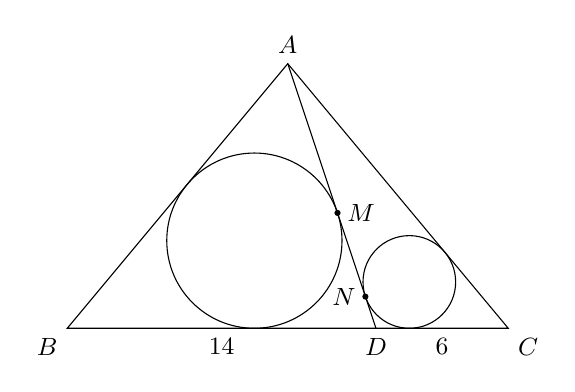
\begin{tikzpicture}[scale=0.28,font=\small]
\coordinate (B) at (0,0); \coordinate (C) at (20,0); \coordinate (A) at (10,12); \coordinate (D) at (14,0);
\coordinate (M) at (12.256,5.231); \coordinate (N) at (13.521,1.437);
\draw (A)--(B)--(C)--cycle; \draw (A)--(D);
\draw (8.486,3.974) circle (3.974); \draw (15.514,2.101) circle (2.101);
\fill (M) circle (4pt); \fill (N) circle (4pt);
\node[above] at (A) {$A$}; \node[below left] at (B) {$B$}; \node[below right] at (C) {$C$}; \node[below] at (D) {$D$};
\node[right] at (M) {$M$}; \node[left] at (N) {$N$}; \node[below] at (7,0) {$14$}; \node[below] at (17,0) {$6$};
\end{tikzpicture}}
\Opts{$2$}{$4$}{$5$}{$8$}}
\QQ{27}{$ABCD$ trapetsiyaning $BC$ va $AD$ asoslari mos ravişda $16$ va $44$ ga, $AB$ va $CD$ yon tomonlari esa mos ravişda $17$ va $25$ ga teng bölsa, $ABCD$ trapetsiya yuzini toping.
\qfig{\begin{tikzpicture}[scale=0.15,font=\small]
\coordinate (A) at (0,0); \coordinate (D) at (44,0); \coordinate (B) at (8,15); \coordinate (C) at (24,15);
\draw (A)--(B)--(C)--(D)--cycle;
\node[below left] at (A) {$A$}; \node[above left] at (B) {$B$}; \node[above right] at (C) {$C$}; \node[below right] at (D) {$D$};
\node[above] at (16,15) {$16$}; \node[below] at (22,0) {$44$}; \node[left] at (4,7.5) {$17$}; \node[right] at (34,7.5) {$25$};
\end{tikzpicture}}
\Opts{$380$}{$450$}{$420$}{$480$}}
\QQ{28}{Muntazam köpburçakning diagonallari soni $35$ ta bölsa, uning bir uçidan çiqqan eng katta va eng kiçik diagonallari orasidagi burçakni toping.
\Opts{$54^\circ$}{$72^\circ$}{$45^\circ$}{$60^\circ$}}
\QQ{29}{$ABCD$ parallelogrammning diagonallari $O$ nuqtada kesişadi. $BC$ tomonda $E$ nuqta şunday olindiki, $\dfrac{BE}{EC}=3$. Agar $\overrightarrow{OE}=a\cdot\overrightarrow{AB}+b\cdot\overrightarrow{BC}$ bölsa, $a+b$ ni toping.
\qfig{\begin{tikzpicture}[scale=0.45,font=\small]
\coordinate (A) at (0,0); \coordinate (B) at (2.5,4); \coordinate (C) at (9.5,4); \coordinate (D) at (7,0); \coordinate (O) at (4.75,2); \coordinate (E) at (7.75,4);
\draw (A)--(B)--(C)--(D)--cycle; \draw (A)--(C); \draw (B)--(D); \draw[-{Stealth[length=5pt]}] (O)--(E); \fill (O) circle (2pt);
\node[below left] at (A) {$A$}; \node[above left] at (B) {$B$}; \node[above right] at (C) {$C$}; \node[below right] at (D) {$D$}; \node[below] at (O) {$O$}; \node[above] at (E) {$E$};
\end{tikzpicture}}
\Opts{$\dfrac12$}{$\dfrac23$}{$\dfrac14$}{$\dfrac34$}}
\QQ{30}{Kesik konusning töla sirti yon sirtidan ikki marta katta. Agar kesik konus asoslarining radiuslari $4$ va $12$ ga teng bölsa, kesik konus hajmini toping.
\Opts{$128\pi$}{$208\pi$}{$416\pi$}{$316\pi$}}
\QQ{31}{Sinfda $25$ ta öquvçi bor. $9$ ta öquvçi kimyo tögaragiga, $8$ ta öquvçi biologiya tögaragiga qatnaşadi. $10$ ta öquvçi esa heç qaysi tögarakka qatnaşmaydi. Neçta öquvçi ikkala tögarakka ham qatnaşadi?
\Opts{$2$}{$3$}{$5$}{$8$}}
\QQ{32}{«MATEMATIKA» sözidagi har bir harf bittadan qoğozga yozib çiqildi. Bitta qoğoz olinganda M harfi çiqiş ehtimolini toping.
\Opts{$\dfrac1{10}$}{$\dfrac3{10}$}{$\dfrac15$}{$\dfrac25$}}
\QQ{33}{\Moslash{Muntazam uçburçakli $SABC$ piramidaning asosining tomoni $2$ ga teng. $AB$ va $BC$ tomonlarining örtalarida $E$ va $D$ nuqtalar olingan. $SED$ kesim asos tekisligi bilan $45^\circ$ li burçak taşkil qiladi.
\par\centering\begin{tikzpicture}[scale=0.85,font=\small]
\coordinate (A) at (0,0); \coordinate (B) at (0.48,2.64); \coordinate (C) at (4.44,1.48); \coordinate (S) at (1.8,4.96); \coordinate (E) at (0.24,1.32); \coordinate (D) at (2.46,2.06);
\fill[qfill] (S)--(E)--(D)--cycle;
\draw (S)--(A)--(C)--cycle; \draw (S)--(B); \draw (A)--(B)--(C); \draw (S)--(E)--(D)--cycle;
\node[below left] at (A) {$A$}; \node[left] at (B) {$B$}; \node[right] at (C) {$C$}; \node[above] at (S) {$S$}; \node[left] at (E) {$E$}; \node[above right] at (D) {$D$};
\end{tikzpicture}}{A) $\dfrac16$\par B) $\dfrac{\sqrt{70}}8$\par C) $\dfrac18$\par D) $\dfrac{\sqrt{15}}6$\par E) $\dfrac1{\sqrt6}$\par F) $\dfrac{\sqrt6}{12}$}{$SD$ uzunligini toping.}{$DES$ kesim yuzini toping.}{$DEACS$ piramida hajmini toping.}}
\QQ{36}{Tenglamani yeçing:
\[x^4-2\sqrt3x^2-x+3-\sqrt3=0\]
\AB{Tenglama neçta musbat ildizga ega?}{Tenglama neçta haqiqiy ildizga ega?}}
\QQ{37}{Tenglamani yeçing:
\[\frac{\tg2x\cdot\tg x}{\tg2x-\tg x}=2\sin\left(\frac\pi4+x\right)\cdot\sin\left(\frac\pi4-x\right)\]
\AB{Tenglamaning eng katta manfiy ildizini toping.}{Tenglamaning $[0;\,\pi]$ oraliqdagi ildizlari sonini toping.}}
\QQ{38}{$f(x)=x^3+ax^2+bx+c$ funksiya berilgan. Agar $(x+1)\cdot f(x-1)+(x-1)\cdot f(x+1)=2x\cdot f(x)$ tenglik örinli bölsa,
\AB{$f(1)-f(-1)$ ning qiymatini toping.}{$f(2)-f(-2)$ ning qiymatini toping.}}
\QQ{39}{Rasmda $(-7;\,9)$ oraliqda $y=f'(x)$ funksiyaning grafigi tasvirlangan ($f'(x)$ — $f(x)$ funksiyaning birinçi tartibli hosilasi, $f''(x)$ — ikkinçi tartibli hosilasi). Grafik $1\times1$ ölçamdagi katakçalarda tasvirlangan.
\qfig{\begin{tikzpicture}[scale=0.38,font=\scriptsize]
\draw[gray!60,dashed] (-8,-5) grid (10,5);
\draw[-{Stealth[length=4pt]}] (-8,0)--(10.6,0) node[right] {$x$}; \draw[-{Stealth[length=4pt]}] (0,-5)--(0,5.6) node[left] {$y$};
\draw[thick] plot[smooth] coordinates {(-7.0,-1.00) (-6.9,-1.22) (-6.8,-1.46) (-6.7,-1.73) (-6.6,-1.99) (-6.5,-2.25) (-6.4,-2.49) (-6.3,-2.69) (-6.2,-2.86) (-6.1,-2.96) (-6.0,-3.00) (-5.9,-2.93) (-5.8,-2.74) (-5.7,-2.45) (-5.6,-2.10) (-5.5,-1.70) (-5.4,-1.29) (-5.3,-0.88) (-5.2,-0.52) (-5.1,-0.21) (-5.0,0.00) (-4.9,0.15) (-4.8,0.27) (-4.7,0.37) (-4.6,0.47) (-4.5,0.55) (-4.4,0.64) (-4.3,0.73) (-4.2,0.83) (-4.1,0.95) (-4.0,1.10) (-3.9,1.31) (-3.8,1.61) (-3.7,1.96) (-3.6,2.35) (-3.5,2.75) (-3.4,3.13) (-3.3,3.47) (-3.2,3.75) (-3.1,3.93) (-3.0,4.00) (-2.9,3.98) (-2.8,3.93) (-2.7,3.85) (-2.6,3.74) (-2.5,3.61) (-2.4,3.45) (-2.3,3.26) (-2.2,3.06) (-2.1,2.85) (-2.0,2.61) (-1.9,2.37) (-1.8,2.11) (-1.7,1.85) (-1.6,1.59) (-1.5,1.32) (-1.4,1.04) (-1.3,0.78) (-1.2,0.51) (-1.1,0.25) (-1.0,0.00) (-0.9,-0.28) (-0.8,-0.63) (-0.7,-1.01) (-0.6,-1.41) (-0.5,-1.81) (-0.4,-2.18) (-0.3,-2.51) (-0.2,-2.77) (-0.1,-2.94) (0.0,-3.00) (0.1,-2.94) (0.2,-2.76) (0.3,-2.50) (0.4,-2.17) (0.5,-1.80) (0.6,-1.40) (0.7,-1.00) (0.8,-0.62) (0.9,-0.28) (1.0,0.00) (1.1,0.25) (1.2,0.52) (1.3,0.78) (1.4,1.05) (1.5,1.30) (1.6,1.53) (1.7,1.72) (1.8,1.87) (1.9,1.97) (2.0,2.00) (2.1,1.97) (2.2,1.87) (2.3,1.72) (2.4,1.53) (2.5,1.30) (2.6,1.05) (2.7,0.78) (2.8,0.52) (2.9,0.25) (3.0,0.00) (3.1,-0.28) (3.2,-0.62) (3.3,-1.00) (3.4,-1.40) (3.5,-1.80) (3.6,-2.17) (3.7,-2.50) (3.8,-2.76) (3.9,-2.94) (4.0,-3.00) (4.1,-2.94) (4.2,-2.79) (4.3,-2.57) (4.4,-2.30) (4.5,-2.00) (4.6,-1.70) (4.7,-1.43) (4.8,-1.21) (4.9,-1.06) (5.0,-1.00) (5.1,-1.03) (5.2,-1.10) (5.3,-1.22) (5.4,-1.35) (5.5,-1.50) (5.6,-1.65) (5.7,-1.78) (5.8,-1.90) (5.9,-1.97) (6.0,-2.00) (6.1,-1.97) (6.2,-1.90) (6.3,-1.78) (6.4,-1.65) (6.5,-1.50) (6.6,-1.35) (6.7,-1.22) (6.8,-1.10) (6.9,-1.03) (7.0,-1.00) (7.1,-1.03) (7.2,-1.10) (7.3,-1.22) (7.4,-1.35) (7.5,-1.50) (7.6,-1.65) (7.7,-1.78) (7.8,-1.90) (7.9,-1.97) (8.0,-2.00) (8.1,-1.99) (8.2,-1.98) (8.3,-1.95) (8.4,-1.92) (8.5,-1.89) (8.6,-1.85) (8.7,-1.81) (8.8,-1.77) (8.9,-1.73) (9.0,-1.70)};
\draw[fill=white] (-7,-1) circle (5pt); \draw[fill=white] (9,-1.7) circle (5pt);
\node[above] at (-7,0) {$-7$}; \node[above] at (9,0) {$9$}; \node[below left] at (0,0) {$O$}; \node[right] at (2.3,3.2) {$y=f'(x)$};
\end{tikzpicture}}
\AB{$y=f(x)$ funksiyaning ekstremum nuqtalari sonini toping.}{$\dfrac{f'(x)}{f''(x)}<0$ tengsizlikni neçta butun son qanoatlantiradi?}}
\QQ{40}{$y=x^3$ funksiyaning grafigi hamda $x=0$ va $y=-1$ töğri çiziqlar bilan çegaralangan soha berilgan ($\pi\approx3$ deb olinsin).
\qfig{\begin{tikzpicture}[scale=1.3,font=\small]
\fill[qfill] (-1,-1)--plot[domain=-1:0,samples=40] (\x,{\x*\x*\x})--(0,-1)--cycle;
\draw[-{Stealth[length=4pt]}] (-1.6,0)--(1.5,0) node[right] {$x$}; \draw[-{Stealth[length=4pt]}] (0,-1.5)--(0,1.5) node[left] {$y$};
\draw[thick,domain=-1.12:1.12,samples=60] plot (\x,{\x*\x*\x}) node[right] {$y=x^3$};
\draw (-1.5,-1)--(0.6,-1) node[right] {$y=-1$};
\node[above left] at (0,0) {$O$}; \node[above] at (-1,0) {$-1$};
\end{tikzpicture}}
\AB{Çegaralangan soha yuzini toping.}{Çegaralangan sohani $Oy$ öqi atrofida $360^\circ$ ga aylantirişdan hosil bölgan jism hajmini toping.}}
\QQ{41}{$ABC$ ($\angle B=90^\circ$) töğri burçakli uçburçakning töğri burçagidan tuşirilgan $BM$ mediana va $BL$ bissektrisa mos ravişda $48$ va $8$ ga teng bölsa,
\qfig{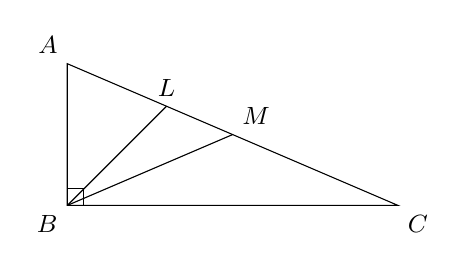
\begin{tikzpicture}[scale=0.6,font=\small]
\coordinate (B) at (0,0); \coordinate (A) at (0,3); \coordinate (C) at (7,0); \coordinate (M) at (3.5,1.5); \coordinate (L) at (2.1,2.1);
\draw (A)--(B)--(C)--cycle; \draw (B)--(M); \draw (B)--(L); \draw (0,0.35)--(0.35,0.35)--(0.35,0);
\node[above left] at (A) {$A$}; \node[below left] at (B) {$B$}; \node[below right] at (C) {$C$}; \node[above right] at (M) {$M$}; \node[above] at (L) {$L$};
\end{tikzpicture}}
\AB{$ABC$ uçburçakning yuzini toping.}{$BML$ uçburçakning yuzini toping.}}
\QQ{42}{$ABCD$ töğri burçakli trapetsiyaning $BC$ kiçik asosi $3$ ga, $AD$ katta asosi $7$ ga, kiçik yon tomoni $AB$ esa $5$ ga teng. Trapetsiyaning diagonallari $O$ nuqtada kesişadi.
\qfig{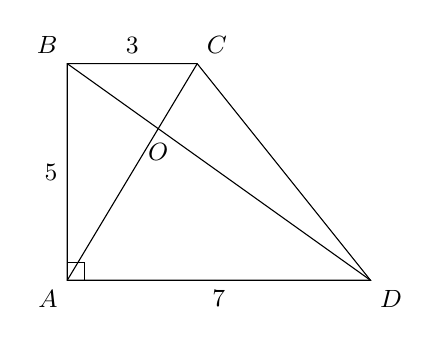
\begin{tikzpicture}[scale=0.55,font=\small]
\coordinate (A) at (0,0); \coordinate (B) at (0,5); \coordinate (C) at (3,5); \coordinate (D) at (7,0); \coordinate (O) at (2.1,3.5);
\draw (A)--(B)--(C)--(D)--cycle; \draw (A)--(C); \draw (B)--(D); \draw (0,0.4)--(0.4,0.4)--(0.4,0);
\node[below left] at (A) {$A$}; \node[above left] at (B) {$B$}; \node[above right] at (C) {$C$}; \node[below right] at (D) {$D$}; \node[below=2pt] at (O) {$O$};
\node[above] at (1.5,5) {$3$}; \node[below] at (3.5,0) {$7$}; \node[left] at (0,2.5) {$5$};
\end{tikzpicture}}
\AB{$O$ nuqtadan kiçik yon tomongaça bölgan eng qisqa masofani toping.}{$COD$ uçburçak yuzini toping.}}
\QQ{43}{$ABCDE$ muntazam beşburçakning $CD$ tomoni örtasida $F$ nuqta olingan. $BD$ diagonal va $AF$ kesma $P$ nuqtada kesişadi.
\qfig{\begin{tikzpicture}[scale=1.25,font=\small]
\coordinate (C) at (0,2); \coordinate (B) at (-1.902,0.618); \coordinate (A) at (-1.176,-1.618); \coordinate (E) at (1.176,-1.618); \coordinate (D) at (1.902,0.618);
\coordinate (F) at (0.951,1.309); \coordinate (P) at (0.449,0.618);
\fill[qfill] (A)--(B)--(P)--cycle;
\draw (A)--(B)--(C)--(D)--(E)--cycle; \draw (B)--(D); \draw (A)--(F);
\draw ($(C)!0.5!(F)+(0.06,0.08)$)--($(C)!0.5!(F)-(0.06,0.08)$); \draw ($(F)!0.5!(D)+(0.06,0.08)$)--($(F)!0.5!(D)-(0.06,0.08)$);
\node[above] at (C) {$C$}; \node[left] at (B) {$B$}; \node[below left] at (A) {$A$}; \node[below right] at (E) {$E$}; \node[right] at (D) {$D$}; \node[above right] at (F) {$F$}; \node[below right] at (P) {$P$};
\node at (1.15,0.85) {$S_1$}; \node at (-0.9,0.0) {$S_2$};
\end{tikzpicture}}
\AB{Agar $|PD|=\sqrt5-1$ bölsa, $BP$ kesma uzunligini toping.}{Agar $S_1=3-\sqrt5$ bölsa, $S_2$ ning qiymatini toping.}}
\QQ{44}{Rasmda markazi $O$ nuqtada, radiusi $10$ ga teng bölgan şar va konus tasvirlangan. Şar va konus $D$ nuqtada urinadi, $AC$ — diametr va $BC=5$ bölsa ($\pi\approx3$ deb olinsin),
\qfig{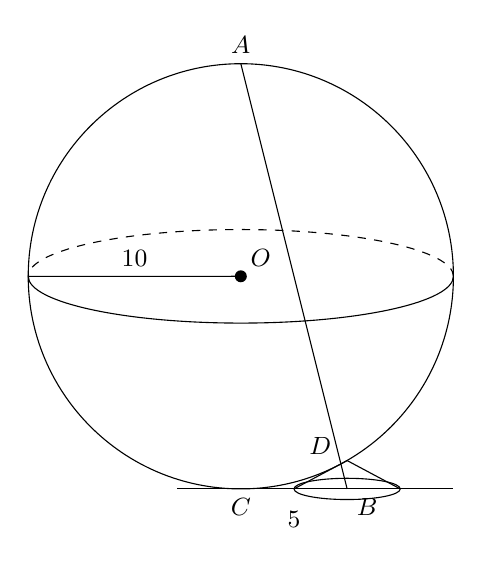
\begin{tikzpicture}[scale=0.27,font=\small]
\coordinate (O) at (0,10); \coordinate (A) at (0,20); \coordinate (C) at (0,0); \coordinate (B) at (5,0); \coordinate (D) at (4.706,1.176); \coordinate (S) at (5,1.333);
\draw (O) circle (10); \draw (-10,10) arc (180:360:10 and 2.2); \draw[dashed] (10,10) arc (0:180:10 and 2.2);
\draw (-3,0)--(10,0); \draw (A)--(B); \draw (O)--(-10,10); \fill (O) circle (8pt);
\draw (B) ellipse (2.5 and 0.5); \draw (2.5,0)--(S)--(7.5,0);
\node[above] at (A) {$A$}; \node[above right] at (O) {$O$}; \node[below] at (C) {$C$}; \node[below right] at (B) {$B$}; \node[above left] at (D) {$D$};
\node[above] at (-5,10) {$10$}; \node[below] at (2.5,-0.6) {$5$};
\end{tikzpicture}}
\AB{Konus asosining radiusini toping.}{Konus balandligini toping.}}
\QQ{45}{Rasmda balandligi $h$ ga teng bölgan bino tasvirlangan. Rasmdagi maʼlumotlardan foydalanib ($\sqrt3\approx1{,}7$ deb olinsin),
\qfig{\begin{tikzpicture}[scale=0.95,font=\small]
\coordinate (A) at (2,2.8); \coordinate (B) at (2,0); \coordinate (C) at (4.8,0); \coordinate (D) at (6.85,0);
\draw (0,0) rectangle (2,2.8);
\foreach \p in {(0.4,1.9),(1.3,1.9),(0.4,1.1),(1.3,1.1)} \draw \p rectangle ++(0.3,0.4);
\draw (0.75,0) rectangle (1.25,0.6); \draw (1,0)--(1,0.6);
\draw[dotted] (-0.5,0)--(7.5,0); \draw[dotted] (A)--(7,2.8);
\draw[dashed] (A)--(C); \draw[dashed] (A)--(D);
\draw (A)++(0:1.6) arc (0:-30:1.6); \node at (3.95,2.55) {$30^\circ$};
\draw (A)++(0:0.9) arc (0:-45:0.9); \node at (3.25,2.0) {$45^\circ$};
\node[above] at (A) {$A$}; \node[below] at (B) {$B$}; \node[below] at (C) {$C$}; \node[below] at (D) {$D$}; \node[right] at (2,1.2) {$h$}; \node[below] at (5.8,0) {$30$};
\end{tikzpicture}}
\AB{Bino balandligini toping.}{$AD$ kesma uzunligini toping.}}
\Javoblar{D A C C B C B A B A A C A C D C A C A A A A D B A B B A D C A C D F C}{\OK{36}{$2$}{$4$}\OK{37}{$-\dfrac{3\pi}8$}{$2$}\OK{38}{$0$}{$12$}\OK{39}{$4$}{$1$}\OK{40}{$\dfrac34$}{$\dfrac95$}\OK{41}{$288$}{$48\sqrt7$}\OK{42}{$\dfrac{21}{10}$}{$\dfrac{21}4$}\OK{43}{$2$}{$4$}\OK{44}{$\dfrac52$}{$\dfrac43$}\OK{45}{$15(\sqrt3+1)\approx40{,}5$}{$30(\sqrt3+1)\approx81$}}
